\section{Introduction}

In our digital world, the demand for computing platforms with higher performance and smaller footprints increases on a daily basis. In later years a class of integrated circuits (ICs) has emerged as the go-to solution for embedded devices where performance, features and small form factor are important parameters, System on Chips (SoCs).

SoCs are fully fledged computer platforms with the necessary memory and storage for operation and powerful peripherals like field programmeable gate arrays (FPGAs) or modems for wireless communication like WiFi, Bluetooth and ZigBee. All of this is packaged on a single chip, thereby the name. In contrast to traditional microcontrollers which has been a favourite in the embedded landscape for decades, SoCs pack a bigger punch. They are equipped with more powerful microprocessors, sometimes even multiprocessors. This makes them a sought after platform for applications where high throughput are crucial, like aerospace, automotive, signal processing, communication, multimedia and military use.

A downside to the increased complexity of the electronics and the demands for smaller devices is the packaging of ICS. Integrated circuits with a high pin count very often use ball grid array (BGA) packages. These are ICs with the connectors placed in a dense grid on the bottom of the packaging, instead of on the tradition side placement. While very space efficient, this way of connecting ICs to printed circuit boards (PCBs) introduces several challenges for hardware designers. Firstly, the clearance between each pin requires PCBs with more than 2 layers. Tradition methods of PCB manufacture like copper etching or milling is only possible (or practical) for 2 layer boards. This means prototypes has to be produced at larger production factories that has the expensive equipment available. Multi-layer boards are also more expensive. It is true that the manufacturing cost and lead time for PCBs has decreased drastically over the last years with the technological advances made, but it still imposes a high cost and increases the time to market. Another important factor is debugging. Advanced multi-layer PCBs are challenging to debug and slows down the development and prototyping phase of product development. Time-to-market is an increasingly important factor when developing embedded systems, as the market is highly competitive and disruptive. 

\subsection{Background}

\subsubsection{Revolve NTNU}

Revolve NTNU is a student organization dedicated to constructing electric formula cars for the international Formula Student competitions. In the course of one year, an electric vehicle (EV) is designed, constructed and tested before entering multiple competitions, facing off against comparable vehicles and teams from other universities from around the world.

\begin{figure}[H]
    \centering
    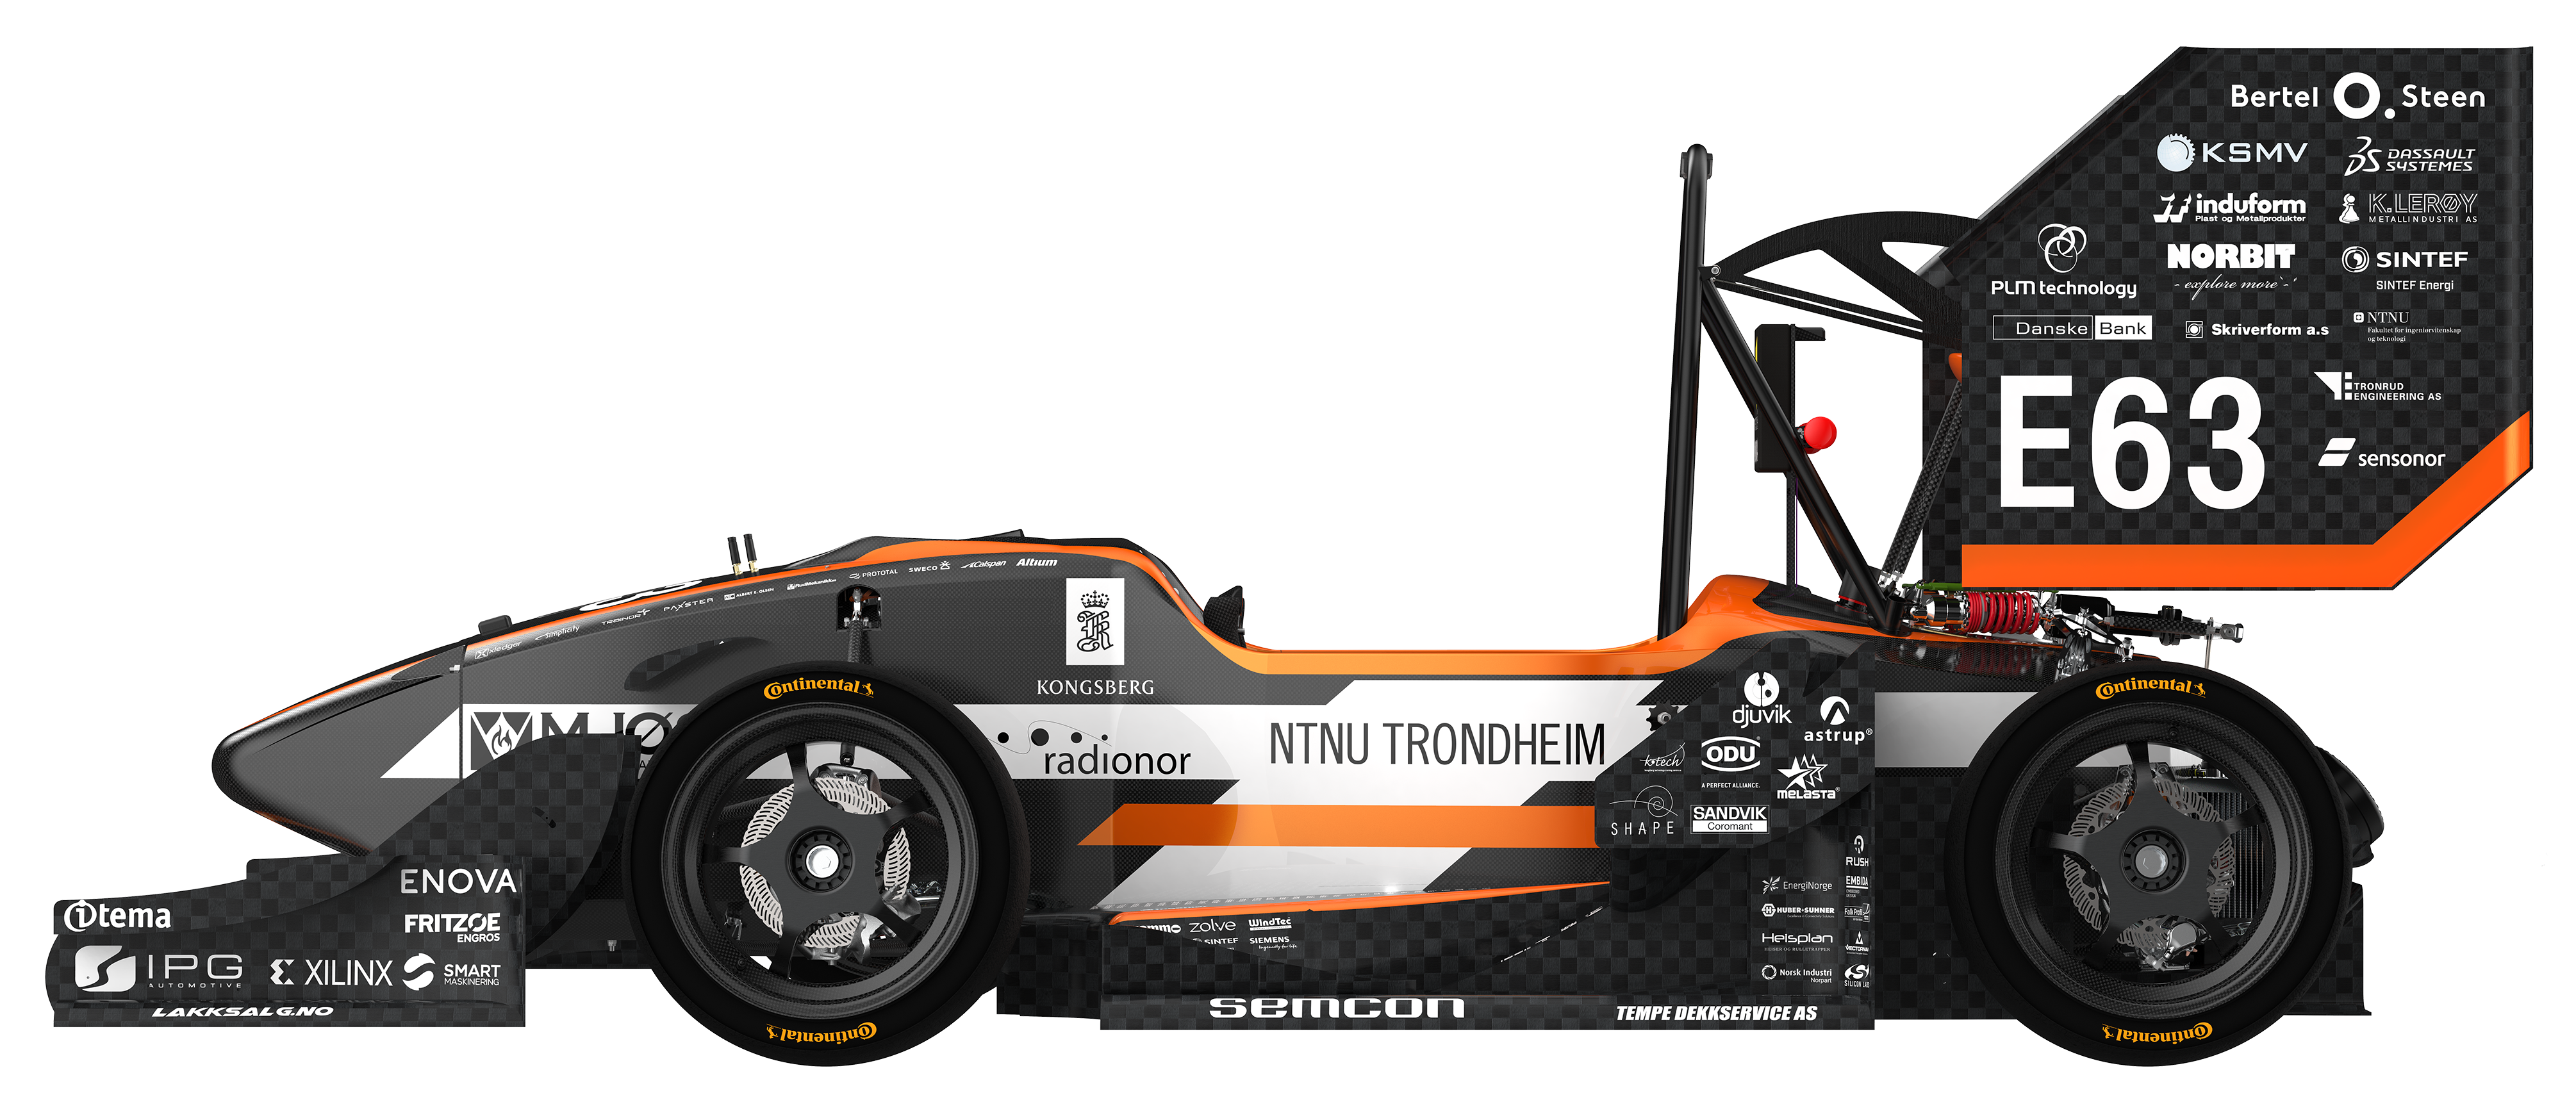
\includegraphics[width=\textwidth]{media/Nova.png}
    \caption{Revolve NTNU 2019's electric vehicle, Nova}
    \label{fig:nova}
\end{figure}

The combination of short development time and a team consisting of mostly new, inexperienced members makes for several interresting problems. This report will focus on a specific embedded system, the vehicle control unit (VCU), and the issues encountered when developing it. As the EV is almost exclusively made from custom parts, the different systems on the car dependends heavily on each other. This means that both changes done the VCU will invariably affect the rest of the vehicle and issues with other systems will most certainly affect the VCU. 

To get a clearer picture of necessary changes to the VCU, we start with the system requirements. analyze last year's VCU, VCU19.

\subsubsection{The vehicle control unit}

The vehicle control unit is the central control system of the electric vehicle. That is, it is responsible for inputting sensory data from the vehicle and the driver, and then output fitting data to electric motors connected to each wheel.

In addition, the VCU is to
\begin{itemize}
    \item put the vehicle into Drive-Enable mode when certain criteria are met
    \item perform safety checks on inputted data and take appropriate action if errors are found
    \item interface with the inertial navigation system (INS)
    \item interface with the data logger provided by competition officials, as per EV 4.6 \cite{fsgrules}
\end{itemize}

The team member responsible for the VCU is not responsible for the implementation of the control algorithms that takes vehicle and driver input and outputs motor set points. The control algorithms performs torque vectoring, a technique for intelligently varying the torque on each wheel {\color{red}(reference here)}, increasing the maneuverability of the EV. The VCU is responsible for providing an environment for the control algorithms to run.

Since the vehicle is capable of speeds exceeding 110 kilometres per hour \cite{novaspeed}, the control algorithms cannot use more time than necessary. As the deadlines the VCU has to uphold are critical for the survival of the vehicle and possibly the driver, it is per definition a \emph{hard real-time embedded system}. However, the exact deadline is unknown. The rule of thmub used by members is that the control loop has to run in at no lower than 100 \si{\hertz}. {\color{red}(Should really find some data on this.)}

\subsubsection{Analysis of VCU19}

To fulfill the requirements of the control algortihm, VCU19 was designed around a new processing platform, the Xilinx Zynq-7000. It is a SoC with a dual core ARM Cortex A9 processor and embedded FPGA \cite{zynq}. There were however issues with this implementation. Advanced processing units like the Zynq-7000 are commonly only available in ball grid array (BGA) packages, meaning packages with all pins placed in a grid pattern on the bottom. This makes hand soldering impossible, a reflow method has to be used instead. This makes assembly and debugging harder, a serious concern considering the rapid development methodologies necessary in Revolve NTNU. The high complexity of design also compelled the previous designer to opt for the smallest available package, a 225 pin BGA package. This limits the available peripherals, but was deemed a necessary compromise during the 2019 season.

\subsection{Analysis of Nova}

As the VCU is an integral part of the EV, issues regarding the vehicle are also issues for the VCU. This section is dedicated to some of the issues encountered during last season, which hopefully can be solved by improving the design of the VCU.

\begin{figure}[h!]
    \centering
    \includegraphics[width=\textwidth]{media/canfd-load.png}
    \caption{CAN-FD bus load}
    \label{fig:canfd_load}
\end{figure}

A major issue with the embedded systems on last years EV is the load on the CAN-FD buses. The vehicle is equipped with 2 buses which are shared between all embedded systems on the car. From the bus load analysis in Figure \ref{fig:canfd_load}, it appears that the first bus has a peak of 80\% load, and the second bus peaks at 70\% when under load. The sudden jump in load on the second bus happens when the vehicle enters \emph{drive enable mode}, i.e. when the VCU starts transmitting data to the inverters that drive the motors. This suggests that data going to and from the VCU accounts for much of the total load on the buses. This can be verified by examining the CAN message overview, see figure ... 

From the aforementioned numbers we can see that much of the data 


\tikzstyle{block}=[draw, thick, minimum size=5mm]

\begin{figure}[h!]
    \centering
    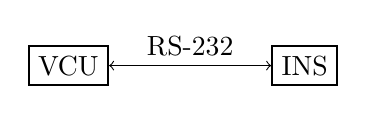
\begin{tikzpicture}[node distance=3cm,auto]
        %Nodes
        \node [block] (vcu) {VCU};
        \node [block] (ins) [right of=vcu] {INS};
        
        %Lines
        \path [<->] (vcu) edge node {RS-232} (ins);
    \end{tikzpicture}
    \caption{CAN-FD bus load}
    \label{fig:canfd}
\end{figure}

\subsection{Scope}

This report covers the design and testing of VCU20. The main focus of the new design is to reduce the complexity of the system while keeping the performance of a SoC. In addition we will take a closer look at the CAN-FD buses connecting the embedded systems on the vehicle.



%\subsection{Interfacing systems}

%The VCU gathers data from other embedded systems on the car. First and foremost we talk about the sonsor broadcasting system (SBS) and the inertial navigation system (INS). 
%\subsubsection{SBS}

%The SBS consists of two equal embedded systems, one placed in the front of the vehicle and one placed in the rear of the vehicle. These boards samples sensor data from and around the wheel and motor assemblies. The SBS's are both connected to the two CAN-FD buses running through the vehicle.

%\subsubsection{INS}

%The INS is an off-the-shelf solution, more precisely a VectorNav VN-300 Rugged. It uses two GPS antennaes, one on the front and one on the main hoop behind the driver, to determine the position, heading, speed and acceleration of the vehicle. The INS has two independent serial interfaces, interface 1 operating on RS-232 voltage levels, and interface 2 operating on TTL voltage levels. The only difference between the two interfaces in terms of functionality is that firmware update of the INS is available through interface 1 only. 

%This, in addition to the higher voltage used on interface 1 making it more resistant to noise, is the reason VCU19 communicated with the INS over interface 1. Note that this requires a TTL to RS-232 level shifter circuit on the VCU.

%\subsubsection{Inverters}

%The inverters converts the DC voltage from the high voltage batteries to a three-phase AC which can be used to drive the electric motors. This is by far the most complex embedded system on the vehicle. It consists of two controller cards, each controlling two inverter power cards. This makes for a total of four motor inverters, one for each motor. The inverter control cards are connected to the two CAN-FD buses, accepting messages containing \emph{set points} for the inverters, meaning how fast each motor shall turn.

%\subsubsection{Telemetry}

%The telemetry system on the vehicle is a long range radio transciever that allows for communication and monitoring of the car from a base station. The radio system is a RadioNor CRE2-144-LW which utilises phase-shift arrays to transmit signals reliably over long distances. The radio interfaces with the vehicle through an Ethernet port, receiving and transmitting UDP packages. In 2019, no other embedded system on the car used Ethernet, and a Respberry Pi 3 B+ was connected to the CAN-FD buses with two PCAN-FD USB dongles so that the embedded systems could interface with the telemetry.

%\subsubsection{Torque vectoring}

%Torque vectoring is the software system that takes the current state of the car and translates this to a desired torque on each of the four motors. It allows for better vehicle handling, especially in turns. It is a software system which should run on the VCU, but the code itself is developed and maintained by another team member. It is therefore crucial that the VCU is capable of running the TV regulation loop at a certain frequency and can supply the required resources (memory and storage). Research shows that the TV control loop has to run at 100Hz minimum to be effective.
 


